\documentclass{beamer}
\usetheme{Copenhagen}
\usefonttheme[onlymath]{serif}
\usepackage{multicol}
\usepackage{graphicx}
\usepackage{hyperref}
\usepackage{float}
\author{Harrison LaBollita}
\institute{Arizona State University}
\title{Kinetic Folder Update}
\date{February 7, 2020}
\logo{
\includegraphics[scale =0.2]{asu.png}}
\definecolor{asu_maroon}{HTML}{8C1D40}
\definecolor{asu_gold}{HTML}{FFC627}
\setbeamercolor{palette primary}{bg=asu_gold,fg=white}
\setbeamercolor{palette secondary}{bg=asu_maroon, fg= white}
\setbeamercolor{palette teritary}{bg=asu_maroon, fg=white}
\setbeamercolor{palette quaternary}{fg=white ,bg=asu_maroon}
\setbeamercolor{navigation symbols}{fg=asu_gold,bg=asu_maroon}
\setbeamercolor{title}{fg=asu_maroon}
\setbeamercolor{frametitle}{fg=asu_maroon}
\setbeamercolor{itemize item}{fg=asu_maroon}
\setbeamertemplate{itemize item}[square]
\begin{document}

\frame{\titlepage}

\section*{Results}
\subsection*{Bad Seq dataset}
\begin{frame}{Results - bad seq dataset}
\begin{itemize}
\item 117 sequences
\item Variable length (max: 80 ntds)
\end{itemize}
\begin{table}
\centering
\begin{tabular}{|ccc|}
\hline
{\bf Stats} & {\bf Kinetic Folder} & {\bf viennaRNA}\\
\hline
\hline
{\bf Mean} & 0.52 & 0.63 \\
{\bf Best} & 0.73 & 0.75 \\
{\bf Worst} & 0.37 & 0.47\\
\hline
\end{tabular}
\end{table}
\end{frame}

\begin{frame}{Results - kinetic folder}
\begin{table}
\centering
\begin{tabular}{|ccc|}
\hline
{\bf Mean} & {\bf Best} & {\bf Worst}\\
\hline
\hline
0.52 & 0.73 & 0.37\\
\hline
\end{tabular}
\end{table}
\begin{figure}[H]
\centering
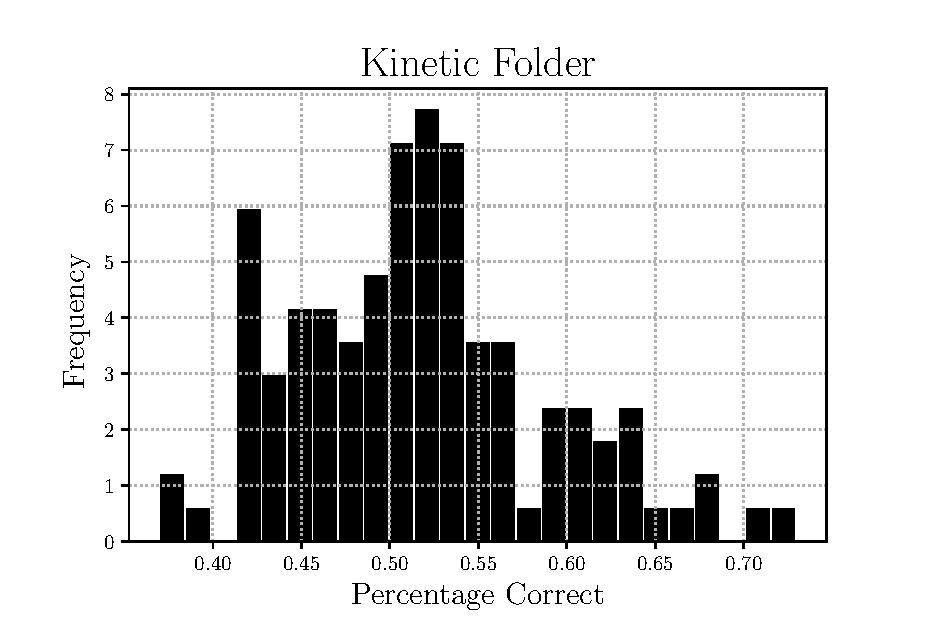
\includegraphics[width = 0.75\textwidth]{myfolder.eps}
\end{figure}
\end{frame}

\begin{frame}{Results - viennaRNA folder}
\begin{table}
\centering
\begin{tabular}{|ccc|}
\hline
{\bf Mean} & {\bf Best} & {\bf Worst}\\
\hline
\hline
0.63 & 0.75 & 0.47\\
\hline
\end{tabular}
\end{table}
\begin{figure}[H]
\centering
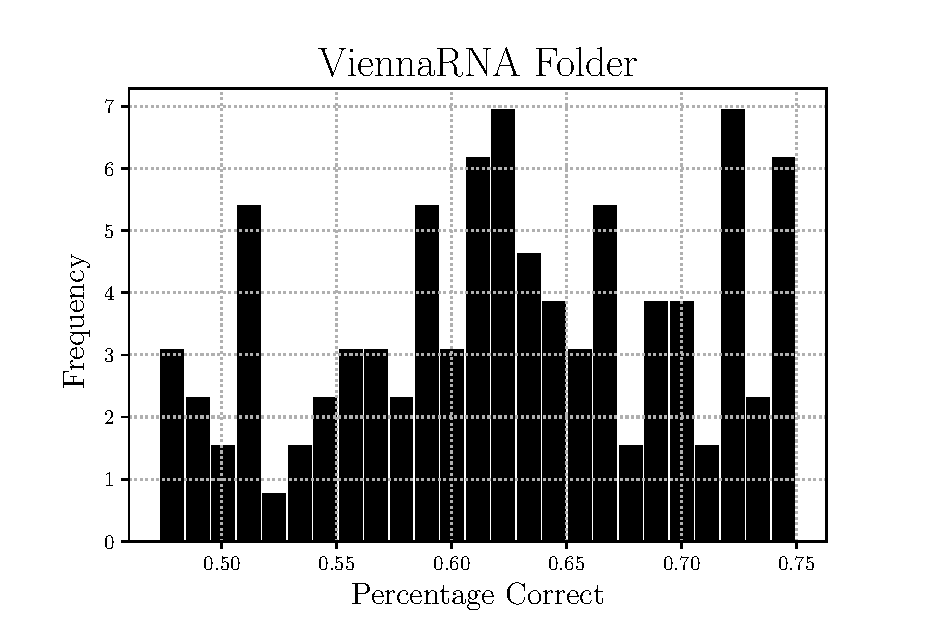
\includegraphics[width = 0.75\textwidth]{viennarna.eps}
\end{figure}
\end{frame}

\subsection*{Pseudoknotted dataset}
\begin{frame}{Results - pseudoknotted}
\begin{itemize}
\item 15 sequences with pseudoknotted secondary structures\footnote{Sequences from \href{http://pseudobaseplusplus.utep.edu}{Pseudobase++} }
\item Mean length: 29 ntds
\end{itemize}
\begin{table}
\centering
\begin{tabular}{|ccc|}
\hline
{\bf Stats} & {\bf Kinetic Folder} & {\bf viennaRNA}\\
\hline
\hline
{\bf Mean} & 0.58 & 0.65 \\
{\bf Best} & 0.93 & 0.77 \\
{\bf Worst} & 0.35 & 0.38\\
\hline
\end{tabular}
\end{table}
\end{frame}

\begin{frame}{Results - kinetic folder}
\begin{table}
\centering
\begin{tabular}{|ccc|}
\hline
{\bf Mean} & {\bf Best} & {\bf Worst}\\
\hline
\hline
0.58 & 0.93 & 0.35\\
\hline
\end{tabular}
\end{table}
\begin{figure}
\centering
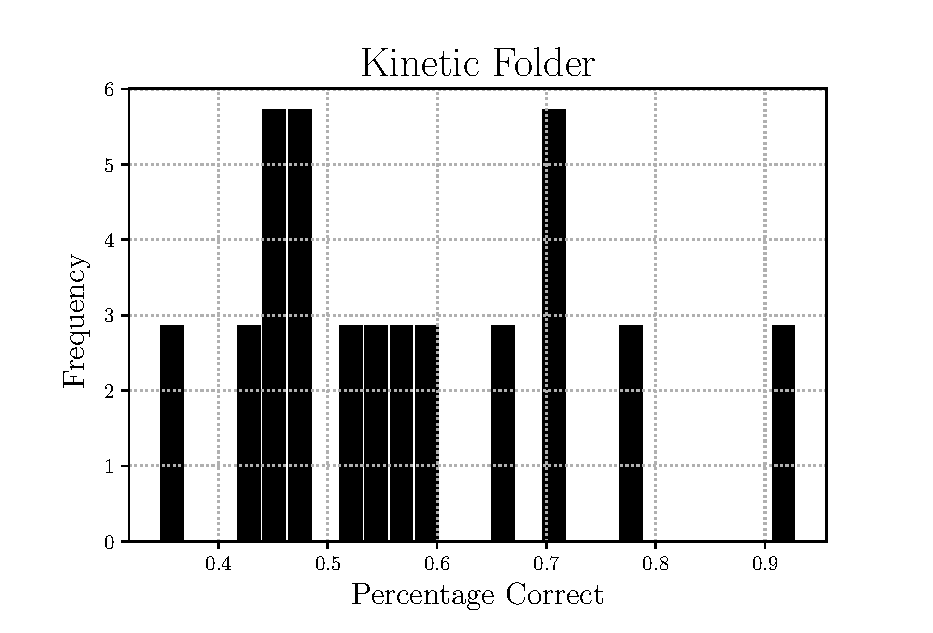
\includegraphics[width =0.75\textwidth]{myfolder_pseudo.eps}
\end{figure}
\end{frame}

\begin{frame}{Results - viennaRNA folder}
\begin{table}
\centering
\begin{tabular}{|ccc|}
\hline
{\bf Mean} & {\bf Best} & {\bf Worst}\\
\hline
\hline
0.65 & 0.77 & 0.38\\
\hline
\end{tabular}
\end{table}
\begin{figure}
\centering
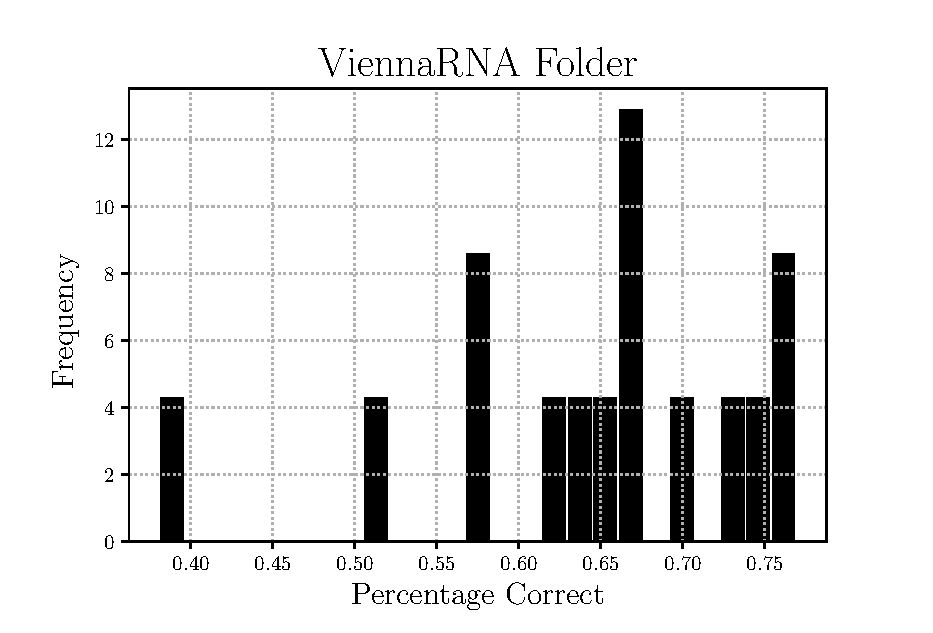
\includegraphics[width =0.75\textwidth]{viennarna_pseudo.eps}
\end{figure}
\end{frame}

\end{document}
